\chapter[Scarefault]{Scarefault}
Neste capítulo será abordado o \Scarefault, o produto final desse
trabalho. Este capítulo está dividido em seções. A primeira seção aborda
uma visão geral do \Scarefault. A segunda seção faz uma análise da
arquitetura do \framework e suas dependências. Na seção seguinte explana-se
a respeito da utilização do \Scarefault.

\section{\Scarefault: Visão Geral}
O \scarefault é um \framework que tem a intenção de gerar testes unitários
de forma semiautomatizada. Para isso, ele necessita da intervenção do
desenvolvedor que o utiliza por meio de breves especificações nos
comentários de documentação. A partir dessas especificações o \scarefault
coleta informações necessárias para a produção dos casos de teste e gera
um arquivo contendo os testes solicitados. É importante ressaltar que,
para esse trabalho, os testes gerados são apenas testes caixa preta.

O \scarefault foi escrito em \cpp e está licenciado dentro das condições
da \textsf{GPLv3}. Todo o seu código fonte encontra-se em:
\url{https://github.com/Scarefault/scarefault}.

\section{A Arquitetura do \scarefault}
Partindo-se de uma visão macroscópica, o \scarefault pode ser dividido em
dois módulos básicos: o \textsf{identificador} e o \textsf{gerador}. A Figura
\ref{modules-scarefault} ilustra esses módulos básicos.

\begin{figure}[h]
  \centering
    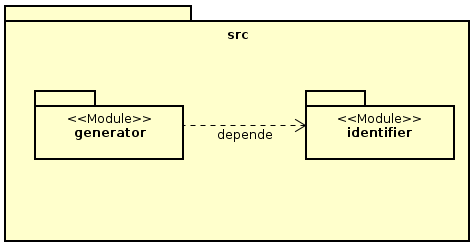
\includegraphics[width=0.6\textwidth]{figuras/modules-scarefault.png}
    \caption{Representação dos módulos do \Scarefault}
    \label{modules-scarefault}
\end{figure}

\begin{description}
\item[Identificador:] é responsável pela identificação das regras que regem
a gramática da linguagem de programação alvo, bem como da coleta dos dados
necessários para a produção dos casos de teste.
\item[Gerador:] responsável pela geração dos casos de teste. A partir dos dados
coletados dos especificações do desenvolvedor e do próprio código fonte, esse
módulo é capaz de gerar casos de teste.
\end{description}

Expandindo-se os módulos pode observar os pacotes associados a cada um deles
e o relacionamento entre esses pacotes, como mostra a Figura
\ref{expand-modules-scarefault-1}.

\begin{figure}[h]
  \centering
    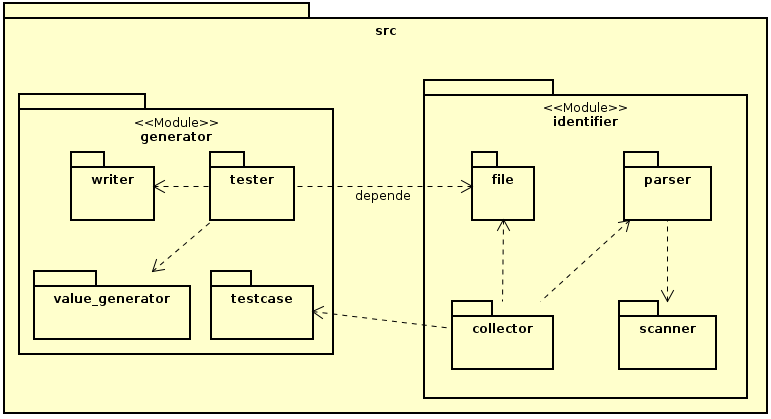
\includegraphics[width=0.8\textwidth]{figuras/expand-modules-scarefault-1.png}
    \caption{Representação expandida dos módulos do \Scarefault}
    \label{expand-modules-scarefault-1}
\end{figure}

\section{A Utilização do \scarefault}